\documentclass[11pt]{article}
\usepackage{amsmath,amsfonts,amssymb} 
\usepackage{mathtools, thmtools}
\usepackage[margin=1in]{geometry}
\usepackage[onehalfspacing]{setspace}
\usepackage{xcolor, graphicx}
\usepackage{caption}
\usepackage{subcaption}
\usepackage[colorlinks, citecolor=blue]{hyperref}
\usepackage[noabbrev, capitalize, nameinlink]{cleveref}
\usepackage{csquotes}

\newtheorem{Theorem}{Theorem}[section]
\newtheorem{Corollary}[Theorem]{Corollary}
\newtheorem{Proposition}[Theorem]{Proposition}
\newtheorem{Lemma}{Lemma}[section]
\newtheorem{Assumption}{Assumption}[section]

\newcommand*{\R}{\mathbb{R}}
\newcommand*{\E}{\mathbb{E}}
\newcommand*{\N}{N}
\newcommand*{\Var}{\mathbb{V}ar}
\newcommand*{\pto}{\stackrel{p}{\to}}
\newcommand*{\dto}{\stackrel{d}{\to}}
\DeclarePairedDelimiter\abs{\lvert}{\rvert}
\DeclarePairedDelimiter\norm{\lVert}{\rVert}
\newcommand{\mvert}[1][\middle]{\ensuremath{\,#1\vert\,}}
\renewcommand{\arraystretch}{1.4}

\usepackage[backend=biber, autopunct=true, authordate, hyperref=true]{biblatex-chicago} 
\addbibresource{riskpriceinference.bib}
\graphicspath{{figures/}}

\author{Xu Cheng  \& Paul Sangrey}
\title{Inference for the Price of Risk Under Weak Identification}
\date{\today}

\begin{document}

\maketitle

First, I start by stating the model taken from  \textcite[Section 5.1]{khrapov2016affine}, which is the model we
will be estimating. 
We will be using spectral GMM, which forms a collection of moment conditions from the characteristic function.
A very quick summary of the idea is as follows. 
Throughout, we will have two key objects of interest the return $r_t$ on some asset and its volatility
$\sigma^2_t$.
I will also follow the convention where time subscripts denote the time when the variable first becomes
observable.
We have a pricing kernel $M_{t, t+1}(\theta)$ which allows us to characterize the price $C_t$ at time $t$ of any
payoff at time $(t+1)$ of some function $H(r_{t+1}, \sigma^2(t+1),  I_t)$. 
I will also use $*$'s to denote the risk neutral measure.

\begin{equation}
    C_t  = \E\left[M_{t,t+1}(\theta) H(r_{t+1}, \sigma^2(t+1),  I_t) \mvert I_t \right] = \E^{*}\left[H(r_{t+1},
    \sigma^2(t+1),  I_t) \mvert I_t \right] 
\end{equation}


To make the problem tractable, we follow \textcite[Section 5.1]{khrapov2016affine} and assume that the problem is
Markov.  
In addition, we assume that there is no Granger causality from return to volatility. 
The conditional probability distribution of $\sigma^2_{t+1} \vert I_t$ equals the conditional probability
distribution of $\sigma^2_{t+1} \vert \sigma_t$.
Consequently, we can write down our model as the following two equations in terms of the Laplace transforms of the
probability distributions, where $a*(u), b*(u)$, and $\alpha{*}(v), \beta^{*}(v), \& \gamma^{*}(v)$ are some
functions.

\begin{align}
    \E^{*}\left[\exp(-x \sigma^2_{t+1}) \mvert \sigma^2_t\right] &= \exp\left(-a^{*}(x) \sigma_t^2 -
    b^{*}(x)\right) \\
    \E^{*}\left[\exp(-x r_{t+1} \mvert \sigma^2_t \sigma^2_{t+1}\right] &= \exp\left(-\alpha^{*}(x) \sigma^2_{t+1}
        - \beta^{*}(x) \sigma^2_t - \gamma^{*}(x)\right)
\end{align}

We are assuming that the volatility follows an autoregressive gamma process (ARG(1).
Hence, its dynamics are determined by following equations.

\begin{gather}
    a(x) = \frac{\rho x}{1 + c x}  \\
    b(x) = \delta \log \left(1 + c x\right) \\
    \rho \in [0, 1), c > 0, \delta > 0 
\end{gather}

The persistence is governed by $\rho$, and the mean by $\delta$, as can be seen by the following equation, while
$c$ is a scaling factor for the volatility. 

\begin{equation}
    \E\left[\sigma^2_{t+1} \mvert \sigma^2_t\right] = c \delta + \rho \sigma^2_t
\end{equation}

Under an assumption that the change of measure preserves the general structure between the risk-neutral and
physical measures, (and possibly some other assumptions).
We end up getting a model for the excess rate formed by the following series of equations.   
We also assume that $\left[ \frac{\psi}{\phi} \right]^2 \approx \frac{\E \left[\sigma^2_{t+1} \mvert
I_t\right]}{\Var\left[r_{t+1} \mvert I_t\right]}$.

\begin{equation}
    \E\left[\exp(-x r_{t+1} \mvert \sigma_t^2, \sigma^2_{t+1}\right] = \exp\left(- a(x) \alpha^2_{t+1} - \beta(x)
        \sigma^2_t - \gamma(x) \right) 
\end{equation}

Then to estimate this equation, we need to fill values for all of the relevant functions.


\begin{align}
    a(x) &= \frac{\rho x}{1 + c x} \\
    b(x) &= \delta \log \left(1 + c x\right) \\
    \alpha(x) &= \psi x - \frac{1}{2} x^2 (1 - \phi^2) \\
    \beta(x)  &= x \alpha^{*}\left(- \frac{\phi}{\sqrt{c [1 + \rho]}} \right) \\
    \gamma(x) &= x b^{*}\left(- \frac{\phi}{\sqrt{c [1 + \rho]}}\right) 
\end{align}

In last two of the above equations we have the risk-neutral $\alpha$ and $\beta$ functions which we have not
defined.
To convert between these two functions, we define the price of volatility risk $\theta_1$ while $\theta_2$
characterizes the price of equity risk. 
The stochastic discount factor satisfies the following equation form some functions $m_0(\cdot)$ and
$m_1(\cdot)$.


\begin{equation}
    M_{t,t+1}(\theta) = \exp(-r_{f,t}) \exp\left(m_{0}(\theta) + m_1(\theta) \sigma_t^2 - \theta_1 \sigma^2_{t+1}
    - \theta_2 r_{t+1}\right)
\end{equation}

Furthermore, the functions $m_0(\cdot)$ and $m_1(\cdot)$ must the exogenously specified dynamics of the risk-free
rate,i.e.\@ the following must hold by the law of iterated expectations.

(Specify the dynamics of $r_{f,t}$.

\begin{equation}
    \E \left[\exp\left(m_{0}(\theta) + m_1(\theta) \sigma_t^2 - \theta_1 \sigma^2_{t+1} - \theta_2 r_{t+1}\right)
    \exp\left(- \alpha(\theta_2) \sigma^2_{t+1} - \beta (\theta_2) \sigma^2_{t+1} - \gamma(\theta_2)\right) \mvert
    I_t \right] = 1
\end{equation}

This implies that we can solve for the two unspecified functions as follows.

\begin{align}
    m_{0}(\theta) &= \gamma(\theta_2) + b\left(\alpha\left(\theta_2\right) + \theta_1\right) \\
    m_{1}(\theta) &= \beta(\theta_2) + a\left(\alpha(\theta_2) + \theta_1\right) 
\end{align}

Now that we have a form for $M_{t,t+1}$ we can solve for $\alpha^{*}(v)$ and $\beta^{*}(v)$. 

\begin{align}
    a^{*}(x) &= a\left(x + \theta_1 + \alpha(\theta_2)\right) - a\left(\theta_1 + \alpha(\theta_2)\right) \\
    b^{*}(x) &= b\left(x + \theta_1 + \alpha(\theta_2)\right) - b\left(\theta_1 + \alpha(\theta_2)\right) \\
\end{align}


We can now substitute them back in to the equations above.


\begin{align}
    a(x) &= \frac{\rho x}{1 + c x} \\ \label{eqn:a(x)}
    b(x) &= \delta \log \left(1 + c x\right) \\ \label{eqn:b(x)}
    \alpha(x) &= x \left(\frac{\phi}{\sqrt{c (1 + \phi)}}  + (1 - \phi^2)\left(\theta_2 - \frac{1}{2}\right)\right)
    - \frac{1}{2} x^2 (1 - \phi^2) \\ \label{eqn:alpha(x)}
    \beta(x)  &= x \left(a\left(-\frac{\phi}{\sqrt{c(1+ \rho)}} + \theta_1 + \alpha(\theta_2)\right) -
        a\left(\theta_1 + \alpha(\theta_2)\right)\right) \\ \label{eqn:beta(x)}
    \gamma(x) &= x \left(b\left(-\frac{\phi}{\sqrt{c(1+\rho)}} + \theta_1 + \alpha(\theta_2)\right) -
        b\left(\theta_1 + \alpha(\theta_2)\right) \right)
\end{align}


Clearly, the set of parameters we want to estimate is $\omega \coloneqq \lbrace c, \rho, \delta, \phi, \theta_1,
\theta_2\rbrace$.

\section{Spectral GMM}

We can derive a set of moment conditions from the characteristic function above by evaluating it a different
points.
That is we can define a function $g_t(u, \text{parameters})$

\begin{equation}
g_t(x, \omega) = Z_t \otimes \begin{bmatrix} \exp(- x \sigma^2_{t+1}) - \exp\left( - a(x) \sigma_t^2 - b(x)
    \right) \\ \exp\left(- x r_{t+1}\right) - \exp\left(- \alpha(x) \sigma^2_{t+1} - \beta(x) \sigma_2^t -
    \gamma(x)\right) \end{bmatrix}
\end{equation}

Where the instruments are given by, for lag order $l = 1, 2$, and complex unit $i$. 

\begin{equation}
    Z_t = \left[1, \exp\left(- i \sigma_t^2\right), \ldots, \exp\left(-i \sigma^2_{t-l}\right)\right] 
\end{equation}

The implied unconditional moment restrictions are the following where $u \in [0,1] \times i [0,1]$.  

\begin{equation}
\E \begin{bmatrix}  \mathrm{Re} (g_t(x, \omega)) \\ \mathrm{Im} (g_t(x, \omega)) \end{bmatrix} = 0
\end{equation}


We want to choose the weighting matrix as the standard covariance matrix of the moment conditions as long as we
choose a finite grid of points for $u$.
If use the entire continuum, we need to handle the weights appropriately.
For now, we will assume that we are only using finitely many moments.

Since the exponential function is a strictly positive function, and we are considering a grid of $x$ values,
a sufficient condition for $\rho, \delta, \& c$ to be identified for $\nabla a(x)$ and $\nabla b(x)$ which are
satisfied if $\rho, c, \delta > 0$.

Seeing if $\phi$ and $\theta_2$ are identified is somewhat trickier. 
Consider the gradient of $\alpha(x)$, again since we are using a grid of $x's$, and the gradient of $\alpha$ is a
nonlinear function of $x$, as long as the gradient is always nonzero, we are identified.

\begin{equation}
    \nabla_{\phi, \theta_2, c}  \alpha(x) = \begin{bmatrix} \phi x^{2} + x \left(- 2 \phi \left(\theta_{2} -
    \frac{1}{2}\right) - \frac{\phi}{2 \sqrt{c} \left(\phi + 1\right)^{\frac{3}{2}}} + \frac{1}{\sqrt{c}
    \sqrt{\phi + 1}}\right) \\ x \left(- \phi^{2} + 1\right) \\ \frac{\phi x}{2 c^{\frac{3}{2}} \sqrt{\phi + 1}}
\end{bmatrix} 
\end{equation}

So $\phi \in (0,1), c > 0$, are sufficient except for the solving the top line for $\theta_2$.
That value, however, is ruled out by derives of $\gamma(x)$, and so does not cause a lack of identification issue.

Identifying, $\theta_1$, is more delicate.

If we plug in the estimated values of the parameters from \textcite{khrapov2016affine}, and plot the derivative
of $\beta(x)$ with respect to $\theta_1$ as a function of $\phi$, we get the following.
The scale is omitted because it is not meaningful. 
As can clearly be seen, there is a zero when $\phi = 0$.

\begin{figure}[htb]
    \centering
    \caption{Derivative of $\gamma(x)$ with respect to $\theta_2$}
    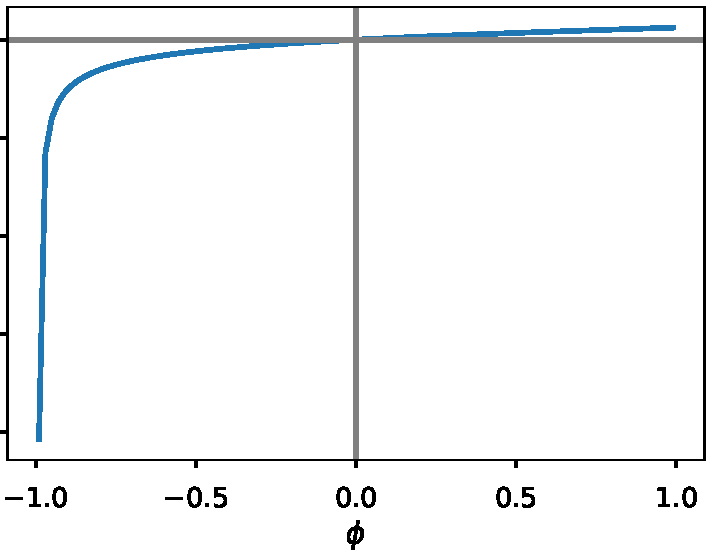
\includegraphics[width=.5\textwidth]{gamma_diff_theta2.pdf}
\end{figure}

The lack of identification is smooth.
%Is this relevant?

For now, we will assume that $\phi \neq 0$, and hence the model is identified.
%And that the derivatives do not cancel out anywhere else.

Hence, clearly for a positive definite weight-matrix by \textcite[Lemma 2.3]{newey1994large} we are identified.
The data $\sigma^2_{t+1}, r_{t+}$ are ergodic and stationary.
If we take the standard GMM estimators of the weight matrix $W$, $\widehat{W}_n \pto W$, and $W$ is positive
semi-definite.  
In addition, clearly $g$ is continuous at each $\omega$, given the restrictions above. 
In addition, properties of characteristic functions imply that $g$ is uniformly bounded. 
For convenience, we will assume that the space of $\omega$, ($\Omega$) is compact.
This should not be an issue here because the parameters  are either a-priori bounded, such as $\phi$ or we have
substantial a-priori knowledge an their plausible magnitudes.
Hence, by \textcite[Theroem 2.6]{newey1994large}, our estimator is consistent.

By the above arguments, we have a consistent estimator for the weight matrix and the parameter, and we will assume
that $\omega_0$ is in the interior of $\Omega$.
Clearly, $g$ is continuously differentiable, and its derivative $G$ is continuous.
In addition, by the identification discussion $G' W G$ is nonsingular.
The only real question is whether $\sqrt{n} g_n(\omega_0) \dto \N(0, \Xi)$ for some matrix $\Xi$.

\begin{Assumption}[Weak Dependence]
    \label{assumption:weak_dependence}
$z_t \coloneqq \begin{pmatrix} r_{t+1} \\ \sigma^2_{t+1} \end{pmatrix}$ are $\alpha$-mixing with $\alpha_n$
    satisfies  $\sum_{n} \alpha_n^{\frac{\delta}{2(2 + \delta)}}$ and $\E\abs*{z_n}^{2+\delta} < \infty $.  
\end{Assumption}

Assume that \cref{assumption:weak_dependence} holds and then by the central limit theorem for strongly mixing
sequences, $\sqrt{n} g_n(\omega_0) \dto \N(0,\Xi)$ as required. 
Consequently, by \textcite[theorem 3.2]{newey1994large} we have convergence in distribution as well as convergence
in probability.


\printbibliography



\end{document}


